% THIS DOCUMENT IS FOLLOWS THE VOLERE TEMPLATE BY Suzanne Robertson and James Robertson
% ONLY THE SECTION HEADINGS ARE PROVIDED
%
% Initial draft from https://github.com/Dieblich/volere
%
% Risks are removed because they are covered by the Hazard Analysis
\documentclass[12pt]{article}

\usepackage{graphicx} 
\graphicspath{ {./res/} }
\usepackage{booktabs}
\usepackage{tabularx}
\usepackage{hyperref}
\hypersetup{
    bookmarks=true,         % show bookmarks bar?
      colorlinks=true,      % false: boxed links; true: colored links
    linkcolor=red,          % color of internal links (change box color with linkbordercolor)
    citecolor=green,        % color of links to bibliography
    filecolor=magenta,      % color of file links
    urlcolor=cyan           % color of external links
}

\newcommand{\lips}{\textit{Insert your content here.}}

%% Comments

\usepackage{color}

\newif\ifcomments\commentstrue %displays comments
%\newif\ifcomments\commentsfalse %so that comments do not display

\ifcomments
\newcommand{\authornote}[3]{\textcolor{#1}{[#3 ---#2]}}
\newcommand{\todo}[1]{\textcolor{red}{[TODO: #1]}}
\else
\newcommand{\authornote}[3]{}
\newcommand{\todo}[1]{}
\fi

\newcommand{\wss}[1]{\authornote{blue}{SS}{#1}} 
\newcommand{\plt}[1]{\authornote{magenta}{TPLT}{#1}} %For explanation of the template
\newcommand{\an}[1]{\authornote{cyan}{Author}{#1}}

%% Common Parts

\newcommand{\progname}{ProgName} % PUT YOUR PROGRAM NAME HERE
\newcommand{\authname}{Team \#, Team Name
\\ Student 1 name
\\ Student 2 name
\\ Student 3 name
\\ Student 4 name} % AUTHOR NAMES                  

\usepackage{hyperref}
    \hypersetup{colorlinks=true, linkcolor=blue, citecolor=blue, filecolor=blue,
                urlcolor=blue, unicode=false}
    \urlstyle{same}
                                


\begin{document}

\title{Software Requirements Specification for \progname: subtitle describing software} 
\author{\authname}
\date{\today}
	
\maketitle

~\newpage

\pagenumbering{roman}

\tableofcontents

~\newpage

\section*{Revision History}

\begin{tabularx}{\textwidth}{p{3cm}p{2cm}X}
\toprule {\textbf{Date}} & {\textbf{Version}} & {\textbf{Notes}}\\
\midrule
Date 1 & 1.0 & Notes\\
Date 2 & 1.1 & Notes\\
\bottomrule
\end{tabularx}

~\\

~\newpage
\section{Purpose of the Project}
\subsection{User Business}
\lips
\subsection{Goals of the Project}
\lips
\section{Stakeholders}
\subsection{Client}
\lips
\subsection{Customer}
\lips
\subsection{Other Stakeholders}
\lips
\subsection{Hands-On Users of the Project}
\lips
\subsection{Personas}
\lips
\subsection{Priorities Assigned to Users}
\lips
\subsection{User Participation}
\lips
\subsection{Maintenance Users and Service Technicians}
\lips

\section{Mandated Constraints}
\subsection{Solution Constraints}
\textbf{Mobile Device}\\
\underline{Description}: User will interact with the system through an app on their mobile device (smartphone).\\
\underline{Rationale}: Mobile devices are widely used and ubiquitous. While at a grocery store, users may need access to the system.\\
\underline{Fit Criterion}: User interface will run entirely on a mobile device.\\
\\
\textbf{Internet access}\\ %%todo: is this too solution specific?
\underline{Description}: User must have internet access.\\
\underline{Rationale}: System servers and databases are used to store collective user data and process that data. User's devices are required to communicate with the servers and databases via internet access.\\
\underline{Fit Criterion}: User interface will have internet access.\\
\\
\textbf{Device with Camera}\\
\underline{Description}: User must be equipped with a device that has a camera. This should be quite common as most smartphones have a camera.\\
\underline{Rationale}: Users will be using the system while they are out on their grocery trips. Thus, the system needs to have a quick and easy method of data input. This also makes it easier for those who have their hands full or do not have the finger mobility to effectively type on their phone keyboards.\\
\underline{Fit Criterion}: System must have access to a mobile camera.\\

\subsection{Implementation Environment of the Current System}
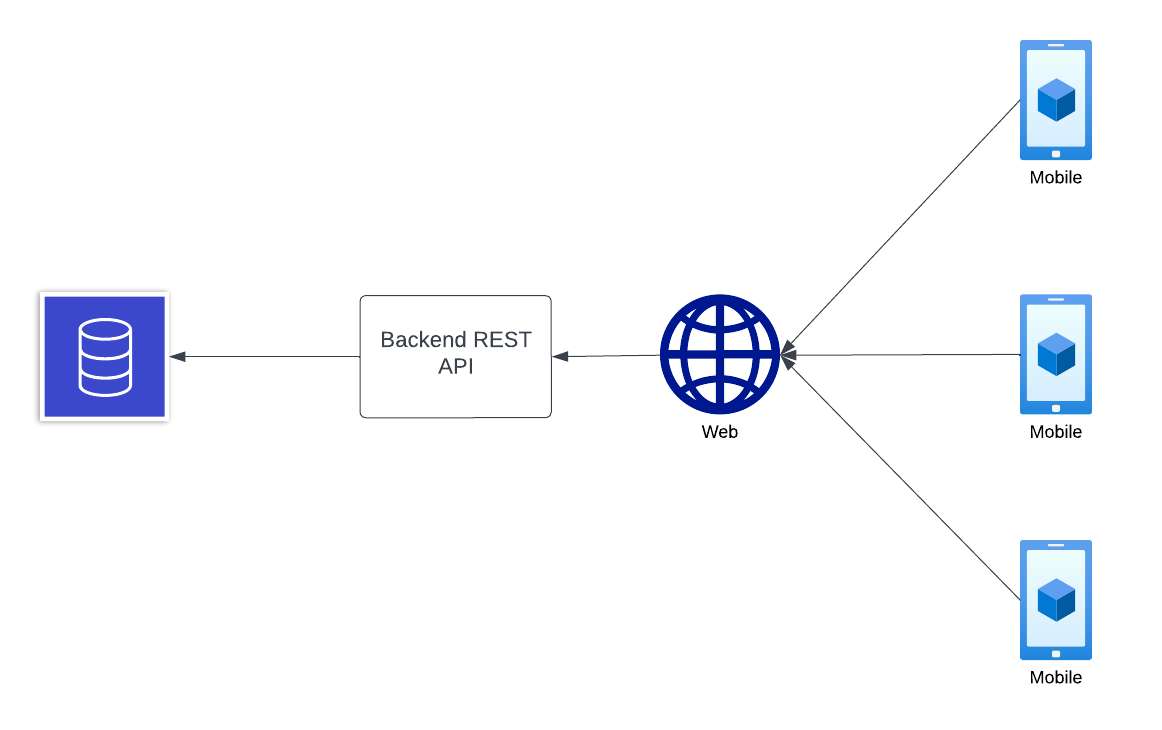
\includegraphics[width=\textwidth]{ImplementationEnvironment.png}

\subsection{Partner or Collaborative Applications}
N/A
\subsection{Off-the-Shelf Software}
The system requires the following off-the-shelf software:
\begin{itemize}
  \item \href{https://github.com/tesseract-ocr/tesseract}{Tesseract} OCR.
  \item \href{https://flutter.dev/}{Flutter} for Front-end.
  \item \href{https://nodejs.org/en}{NodeJS} for Back-end.
  \item \href{https://www.npmjs.com/package/express}{Express} REST API.
  \item \href{https://www.postgresql.org/}{PostgreSQL} as Relational Database.
\end{itemize}

\subsection{Anticipated Workplace Environment}
N/A
\subsection{Schedule Constraints}
The schedule for this project is in adherance with the milestones implemented by our course instructor. Found \href{https://gitlab.cas.mcmaster.ca/courses/capstone/-/blob/main/CourseOutline/Capstone_Outline.pdf}{here}.
\subsection{Budget Constraints}
The project budget is \$750 paid for directly by the developers.
\subsection{Enterprise Constraints}
N/A
\section{Naming Conventions and Terminology}
\subsection{Glossary of All Terms, Including Acronyms, Used by Stakeholders
involved in the Project}
\lips

\section{Relevant Facts And Assumptions}
\subsection{Relevant Facts}
\lips
\subsection{Business Rules}
\lips
\subsection{Assumptions}
\lips

\section{The Scope of the Work}
\subsection{The Current Situation}
\lips
\subsection{The Context of the Work}
\lips
\subsection{Work Partitioning}
\lips
\subsection{Specifying a Business Use Case (BUC)}
\lips

\section{Business Data Model and Data Dictionary}
\subsection{Business Data Model}
\lips
\subsection{Data Dictionary}
\lips

\section{The Scope of the Product}
\subsection{Product Boundary}
\lips
\subsection{Product Use Case Table}
\lips
\subsection{Individual Product Use Cases (PUC's)}
\lips

\section{Functional Requirements}
\subsection{Functional Requirements}
\lips

\section{Look and Feel Requirements}
\subsection{Appearance Requirements}
\lips
\subsection{Style Requirements}
\lips

\section{Usability and Humanity Requirements}
\subsection{Ease of Use Requirements}
\lips
\subsection{Personalization and Internationalization Requirements}
\lips
\subsection{Learning Requirements}
\lips
\subsection{Understandability and Politeness Requirements}
\lips
\subsection{Accessibility Requirements}
\lips

\section{Performance Requirements}
\subsection{Speed and Latency Requirements}
\lips
\subsection{Safety-Critical Requirements}
\lips
\subsection{Precision or Accuracy Requirements}
\lips
\subsection{Robustness or Fault-Tolerance Requirements}
\lips
\subsection{Capacity Requirements}
\lips
\subsection{Scalability or Extensibility Requirements}
\lips
\subsection{Longevity Requirements}
\lips

\section{Operational and Environmental Requirements}
\subsection{Expected Physical Environment}
\lips
\subsection{Wider Environment Requirements}
\lips
\subsection{Requirements for Interfacing with Adjacent Systems}
\lips
\subsection{Productization Requirements}
\lips
\subsection{Release Requirements}
\lips

\section{Maintainability and Support Requirements}
\subsection{Maintenance Requirements}
\lips
\subsection{Supportability Requirements}
\lips
\subsection{Adaptability Requirements}
\lips

\section{Security Requirements}
\subsection{Access Requirements}
\lips
\subsection{Integrity Requirements}
\lips
\subsection{Privacy Requirements}
\lips
\subsection{Audit Requirements}
\lips
\subsection{Immunity Requirements}
\lips

\section{Cultural Requirements}
\subsection{Cultural Requirements}
\lips

\section{Compliance Requirements}
\subsection{Legal Requirements}
\lips
\subsection{Standards Compliance Requirements}
\lips

\section{Open Issues}
\lips

\section{Off-the-Shelf Solutions}
\subsection{Ready-Made Products}
\lips
\subsection{Reusable Components}
\lips
\subsection{Products That Can Be Copied}
\lips

\section{New Problems}
\subsection{Effects on the Current Environment}
\lips
\subsection{Effects on the Installed Systems}
\lips
\subsection{Potential User Problems}
\lips
\subsection{Limitations in the Anticipated Implementation Environment That May
Inhibit the New Product}
\lips
\subsection{Follow-Up Problems}
\lips

\section{Tasks}
\subsection{Project Planning}
\lips
\subsection{Planning of the Development Phases}
\lips

\section{Migration to the New Product}
\subsection{Requirements for Migration to the New Product}
\lips
\subsection{Data That Has to be Modified or Translated for the New System}
\lips

\section{Costs}
\lips
\section{User Documentation and Training}
\subsection{User Documentation Requirements}
\lips
\subsection{Training Requirements}
\lips

\section{Waiting Room}
\lips

\section{Ideas for Solution}
\lips

\newpage{}
\section*{Appendix --- Reflection}

The information in this section will be used to evaluate the team members on the
graduate attribute of Lifelong Learning.  Please answer the following questions:

\begin{enumerate}
  \item What knowledge and skills will the team collectively need to acquire to
  successfully complete this capstone project?  Examples of possible knowledge
  to acquire include domain specific knowledge from the domain of your
  application, or software engineering knowledge, mechatronics knowledge or
  computer science knowledge.  Skills may be related to technology, or writing,
  or presentation, or team management, etc.  You should look to identify at
  least one item for each team member.
  \item For each of the knowledge areas and skills identified in the previous
  question, what are at least two approaches to acquiring the knowledge or
  mastering the skill?  Of the identified approaches, which will each team
  member pursue, and why did they make this choice?
\end{enumerate}

\end{document}